
% \subsection{Statement of the received results and their analysis}



\subsection{MMS 1}

(insert table instead of equations, check comments in tex file for parameters)
\begin{table}[h!]
    \centering
    \begin{tabular}{c|r}
        $\bar{A}$ & test
    \end{tabular}
    \caption{Manufactured solution table for the first MMS test case}
    \label{tab:MMS1_input}
\end{table}
% \begin{equation}
%     M_x = 0.3 \left(
%     \sum_{j=1}^5 R_{ij} +
%     \sum_{j=1}^5 L_{ij} + 1
%     \right) , B = 50
%     \label{eqn:MMS_M_x}
% \end{equation}

% \begin{equation}
%     \tilde{A} = \left(
%     \sum_{j=1}^5 R_{ij} +
%     \sum_{j=1}^5 L_{ij} + 1
%     \right) , B = 0.3
%     \label{eqn:MMS_A}
% \end{equation}

% \begin{align}
%     \tilde{v}_{r,BCsImposed} = 
%     \sum_{j=1}^3 R_{ij} +
%     \sum_{j=1}^3 L_{ij} + 1, \\
%     B = 2 , \\ 
%     \tilde{v}_{r,BCsImposed}(\tilde{r}_{min}=\tilde{r}_{max}) = 0
%     \label{eqn:MMS_vTh}
% \end{align}

% \begin{equation}
%     \tilde{v}_{\theta} = \left(
%     \sum_{j=1}^4 R_{ij} +
%     \sum_{j=1}^4 L_{ij} + 1
%     \right) , B = 50 
%     \label{eqn:MMS_vTh}
% \end{equation}

% \begin{equation}
%     \tilde{v}_{x} = 
%     \sum_{j=1}^3 R_{ij} +
%     \sum_{j=1}^3 L_{ij} + 1
%     , B = 30 
%     \label{eqn:MMS_vX}
% \end{equation}

% \begin{align}
%     \tilde{p}_{diffBCsImposed} = 
%     \sum_{j=1}^5 R_{ij} +
%     \sum_{j=1}^5 L_{ij} + 1
%     , B = 30 
%     \label{eqn:MMS_p}
% \end{align}

Figure \ref{fig:1} shows the manufactured solution for the mean flow profile. The tangent
summation method was used to generate the axial Mach number, the speed of sound, and the perturbation variables. The tangential Mach number was numerically
approximated by using the composite trapezoidal rule. The manufactured mean flow
profile is unique because it has been generated solely to verify SWIRL
and does not have physical significance. The “kinks” in the solution will allow a significant magnitude for the derivatives of these solutions.
\begin{figure}[h!]
    \centering
    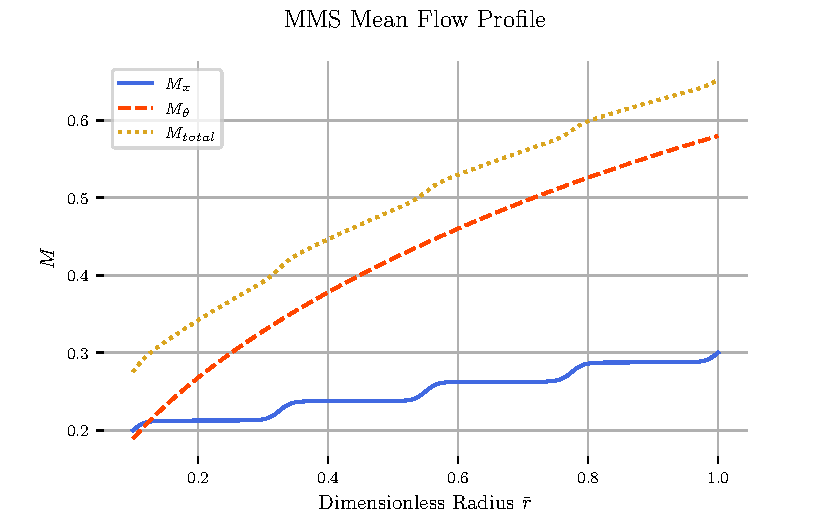
\includegraphics{/home/jeff-severino/SWIRL/CodeRun/04-plotReport/tex-outputs/MMS1_mean_flow_profile.pdf}
    \caption{The manufactured mean flow test case using a summation of Tangents for $A$ and $M_x$}
    \label{fig:1}
\end{figure}
The results from the numerical integration are presented in Figure \ref{fig:5}. Although
the slope of the line appears linear, the TSM was still used to generate the MS for
the speed of sound. Denser grids were used to compute the error by iterating as grid spacing approaches zero. The difference
between the expected speed of sound to the actual speed of sound is shown in Figure
\ref{fig:5a} as a function of radius. Note that the error reaches machine precision early in the iterations and approaches zero as more grid points are used.
\begin{figure}[h!]
    \centering
    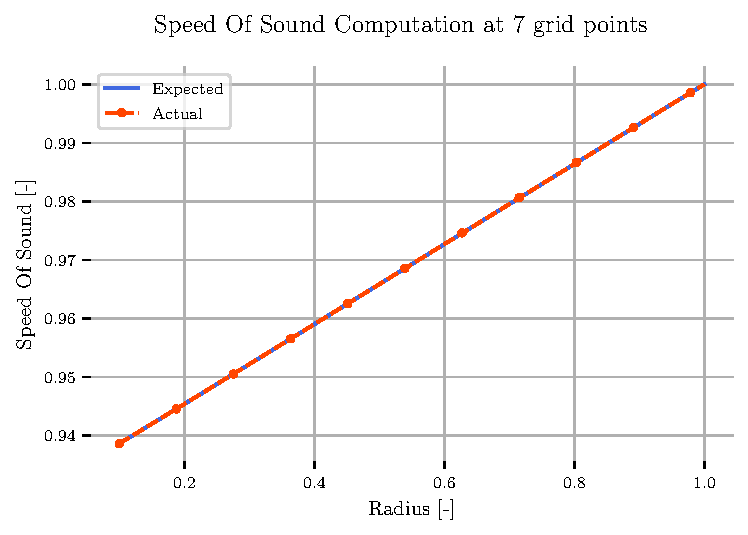
\includegraphics{/home/jeff-severino/SWIRL/CodeRun/04-plotReport/tex-outputs/MMS1_SpeedOfSoundComparison1.pdf}
    \caption{ A comparison of the speed of sound, expected vs actual at the lowest grid to show similarities in solution}
    \label{fig:5}
\end{figure}


\begin{figure}[h!]
    \centering
    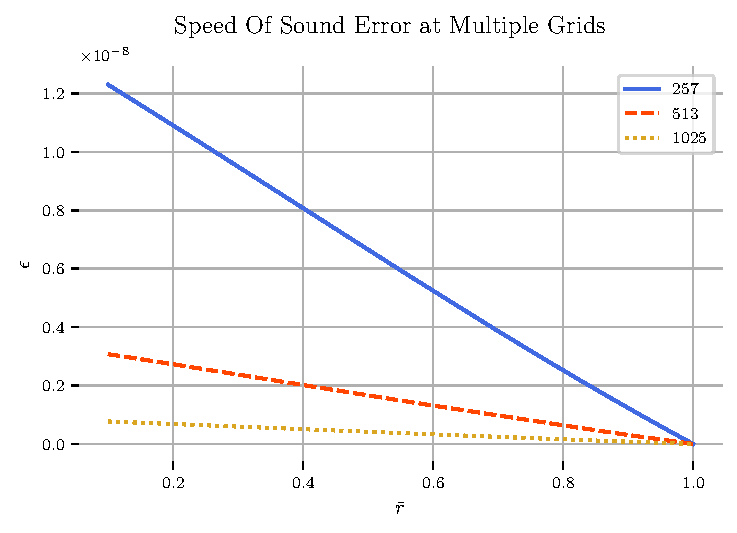
\includegraphics{/home/jeff-severino/SWIRL/CodeRun/04-plotReport/tex-outputs/MMS1_SpeedOfSoundComparison2.pdf}
    \caption{ A comparison of the speed of sound error at three grid}
    \label{fig:5a}
\end{figure}
The error will decrease at a known rate depending on the type of numerical integration scheme. Since the composite trapezoidal rule has an order of accuracy
of 2, it is expected that the approximated order of accuracy will approach two as the
error approaches zero. This behavior is shown in Figure \ref{fig:8}, where the approximated
line is the L2 norm of the speed of sound error. The slope (i.e., the asymptotic rate of
convergence) approached two for numerical integration as the grid spacing decreases
(See Figure \ref{fig:9}) .

\begin{figure}[h!]
    \centering
    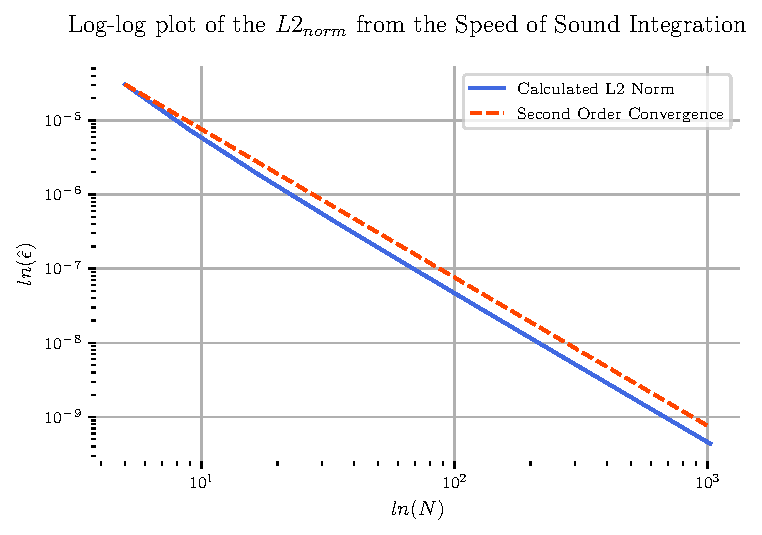
\includegraphics{/home/jeff-severino/SWIRL/CodeRun/04-plotReport/tex-outputs/MMS1_SpeedOfSoundComparisonL2.pdf}
    \caption{L2 Norm comparison for the speed of sound integration for the compound trapezoidal rule}
    \label{fig:8}
\end{figure}

The manufactured solution used for the fluctuation variables in the MMS test case
is shown in Table \ref{tab:MMS1_input}. Recall that the variable B varies the slope around the
tangent function at each inflection point; the maximum amplitude of each tangent
function was A = 0.1 and was equally spaced between $\tilde{r}_{min}$-$\tilde{r}_{max}$.  
The boundary conditions for the perturbation variable $\tilde{v}_r$ were set 
using the fairing functions to impose boundary conditions. Fairing functions 
also set the derivative of the perturbation variable $\tilde{p}$. Only $\tilde{p}$
is affected by acoustic liners since it alters the rate of change of pressure at 
the walls, not the pressure or velocity. The subscripts $BCsImposed, diffBCsImposed$
state where the perturbation or its derivative value was altered to be uniform between the code and
the manufactured solution.


\begin{figure}[h!]
    \centering
    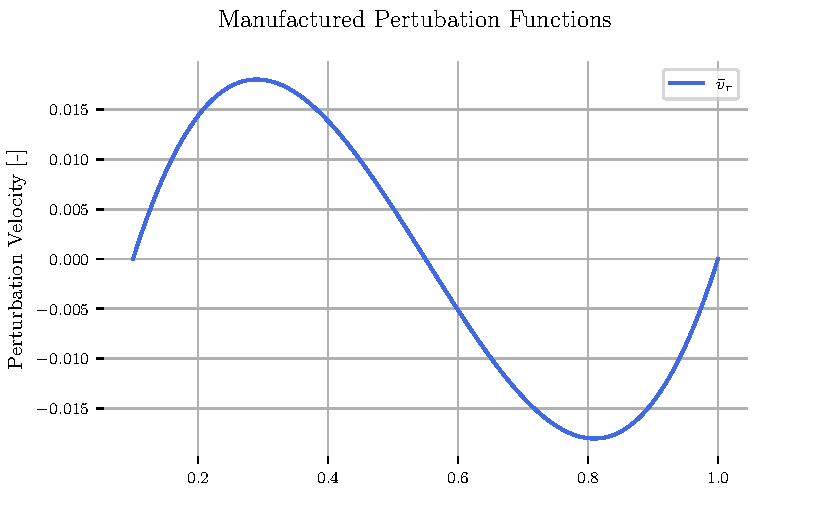
\includegraphics{/home/jeff-severino/SWIRL/CodeRun/04-plotReport/tex-outputs/MMS1_perturbation_variables_vR.pdf}
\caption{The manufactured perturbation functions ,$v_r$}%, $v_x$, $v_{\theta}$, $p$}
    \label{fig:1a}
\end{figure}


\begin{figure}[h!]
    \centering
    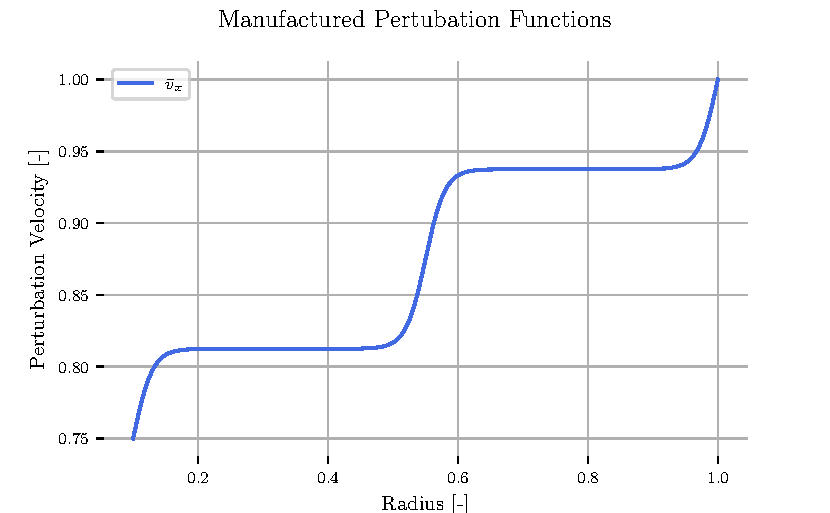
\includegraphics{/home/jeff-severino/SWIRL/CodeRun/04-plotReport/tex-outputs/MMS1_perturbation_variables_vX.pdf}
\caption{The manufactured perturbation functions ,$v_x$}%, $v_x$, $v_{\theta}$, $p$}
    \label{fig:2a}
\end{figure}


\begin{figure}[h!]
    \centering
    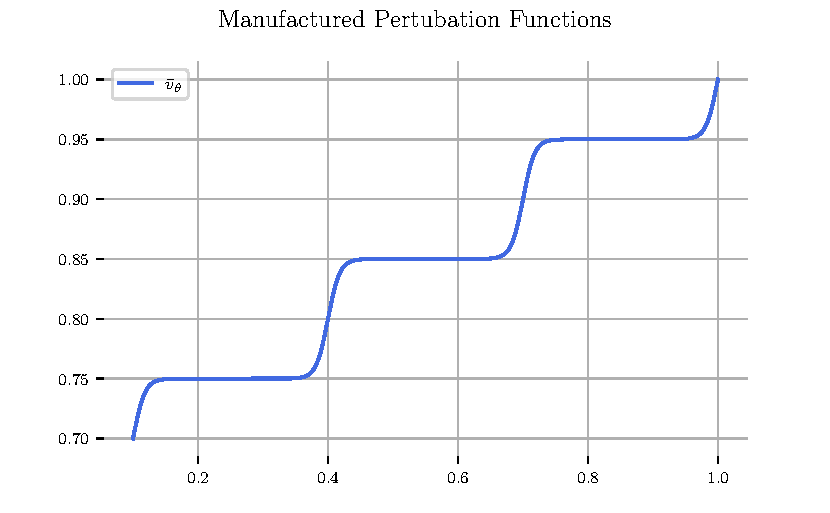
\includegraphics{/home/jeff-severino/SWIRL/CodeRun/04-plotReport/tex-outputs/MMS1_perturbation_variables_vTh.pdf}
    \caption{The manufactured perturbation functions ,$v_{\theta}$}%, $v_x$, $v_{\theta}$, $p$}
    \label{fig:3a}
\end{figure}


\begin{figure}[h!]
    \centering
    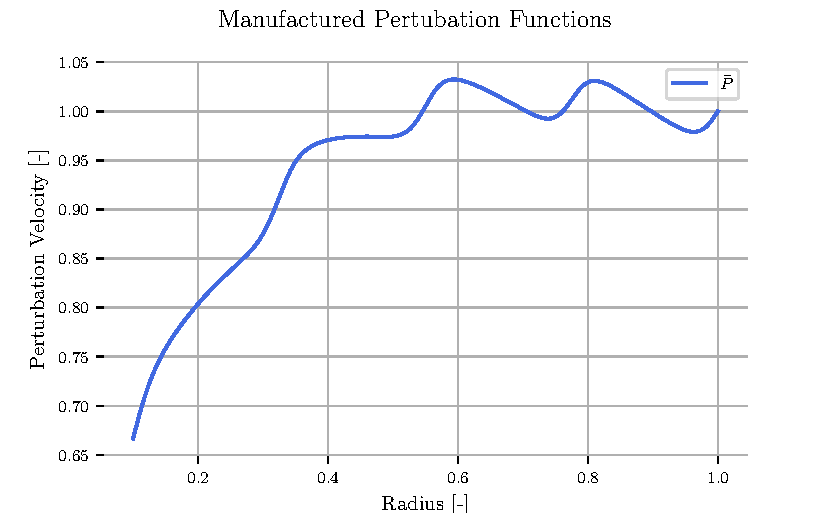
\includegraphics{/home/jeff-severino/SWIRL/CodeRun/04-plotReport/tex-outputs/MMS1_perturbation_variables_Pr.pdf}
\caption{The manufactured perturbation functions ,$P$}%, $v_x$, $v_{\theta}$, $p$}
    \label{fig:4a}
\end{figure}



A second and fourth-order central differencing scheme for the LEE is used for the approximated radial derivatives and compared to the source terms generated for the MMS in Figure 5-10.The L2 norm and the asymptotic rate of convergence is shown for the two diffferencing schemes in 5-15 and ??. 

The grid points were doubled, starting at 7 grid points and ending after 9 iterations with 1025 grid points. Both schemes do not have the order of accuracy down to machine precision but get down to $10^-6$
For the LEE, a second and fourth order central differencing scheme is used
for the approximated radial derivatives and then compared to the source terms 
generated for the MMS in Figure \ref{fig:6}. 
\begin{figure}[h!]
    \centering
    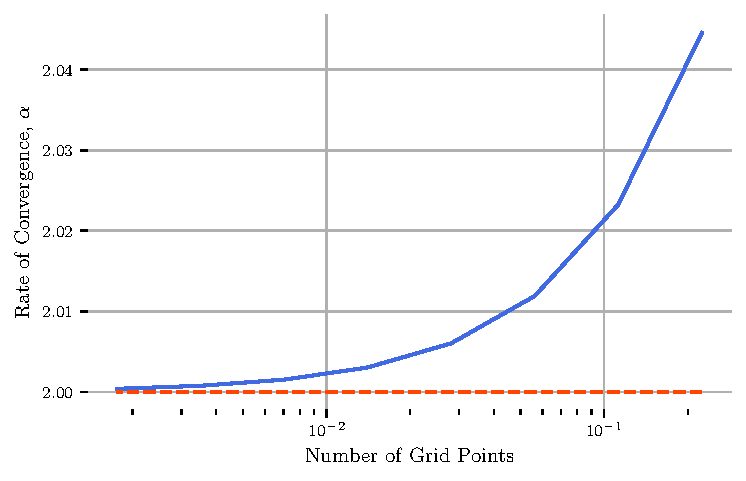
\includegraphics{/home/jeff-severino/SWIRL/CodeRun/04-plotReport/tex-outputs/MMS1_SpeedOfSoundComparisonROC.pdf}
    \caption{ Speed of Sound Rate Of Convergence}
    \label{fig:SpeedOfSoundROC}
\end{figure}



\begin{figure}[h!]
    \centering
    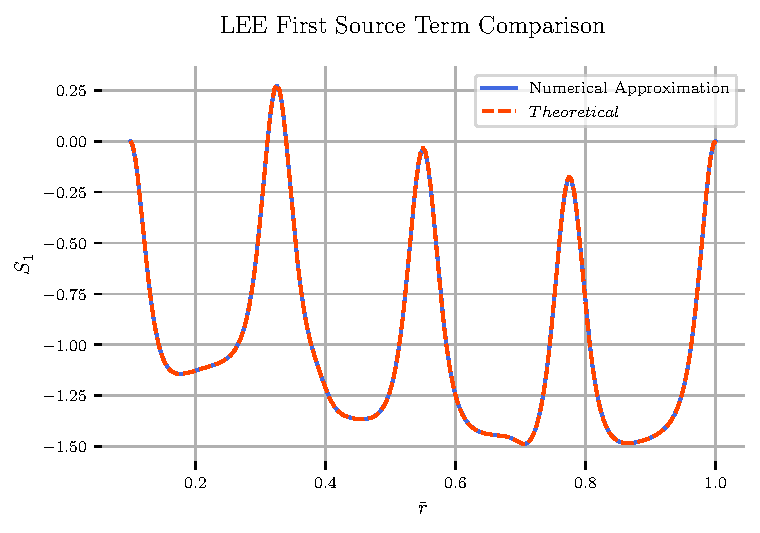
\includegraphics{/home/jeff-severino/SWIRL/CodeRun/04-plotReport/tex-outputs/MMS1_SourceTermComparison1.pdf}
    \caption{LEE Source Terms}
    \label{fig:6}
\end{figure}


\begin{figure}[h!]
    \centering
    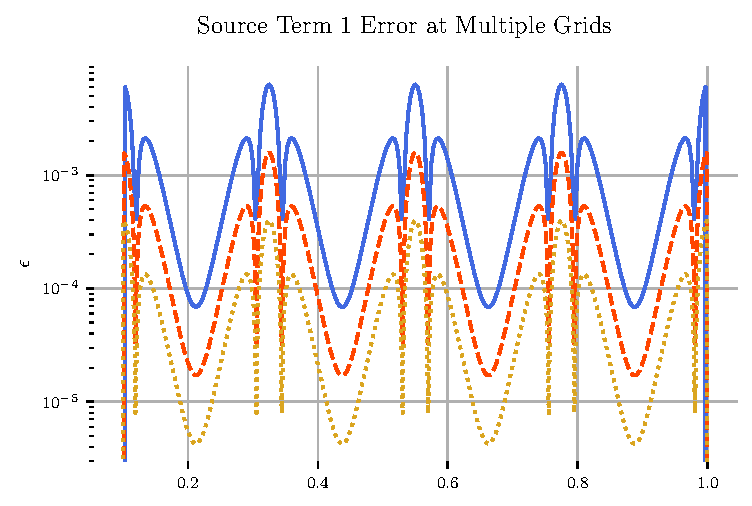
\includegraphics{/home/jeff-severino/SWIRL/CodeRun/04-plotReport/tex-outputs/MMS1_SourceTermError1.pdf}
    \caption{LEE Source Term Error}
    \label{fig:7}
\end{figure}


\begin{figure}[h!]
    \centering
    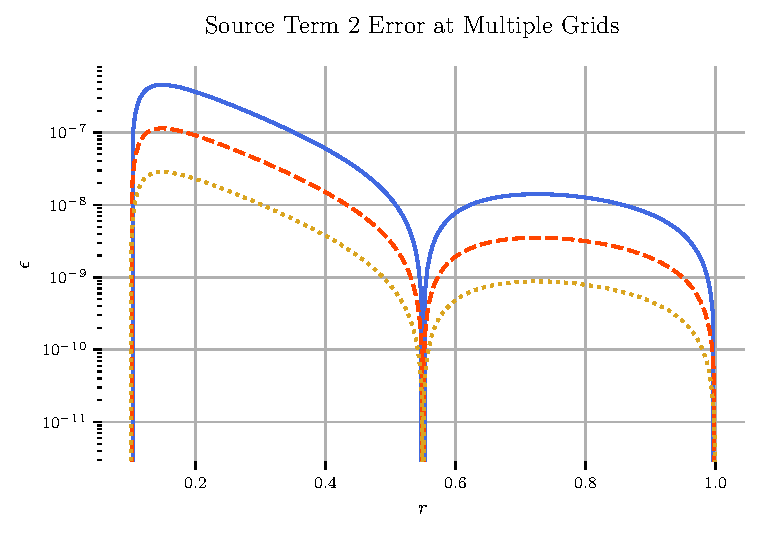
\includegraphics{/home/jeff-severino/SWIRL/CodeRun/04-plotReport/tex-outputs/MMS1_SourceTermError2.pdf}
    \caption{LEE Source Term Error}
    \label{fig:7}
\end{figure}


\begin{figure}[h!]
    \centering
    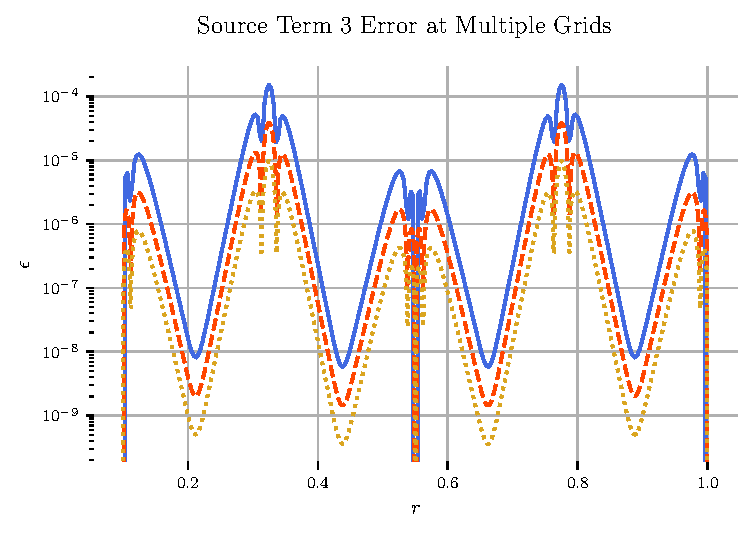
\includegraphics{/home/jeff-severino/SWIRL/CodeRun/04-plotReport/tex-outputs/MMS1_SourceTermError3.pdf}
    \caption{LEE Source Term Error}
    \label{fig:7}
\end{figure}


\begin{figure}[h!]
    \centering
    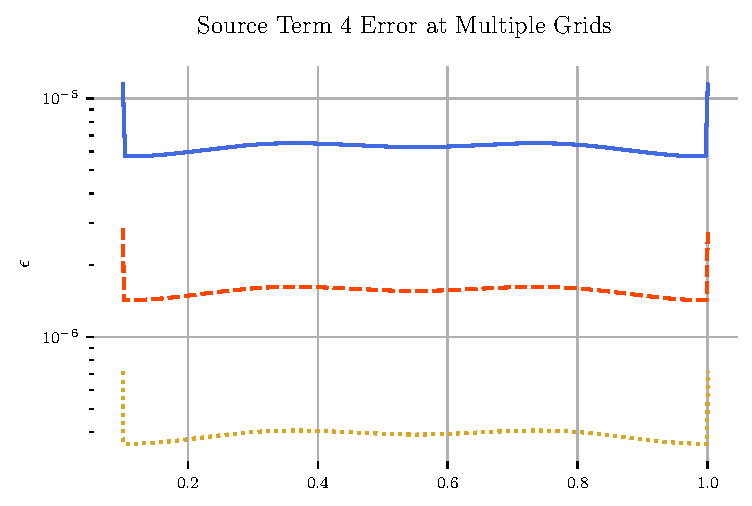
\includegraphics{/home/jeff-severino/SWIRL/CodeRun/04-plotReport/tex-outputs/MMS1_SourceTermError4.pdf}
    \caption{LEE Source Term Error}
    \label{fig:7}
\end{figure}


\begin{figure}[h!]
    \centering
    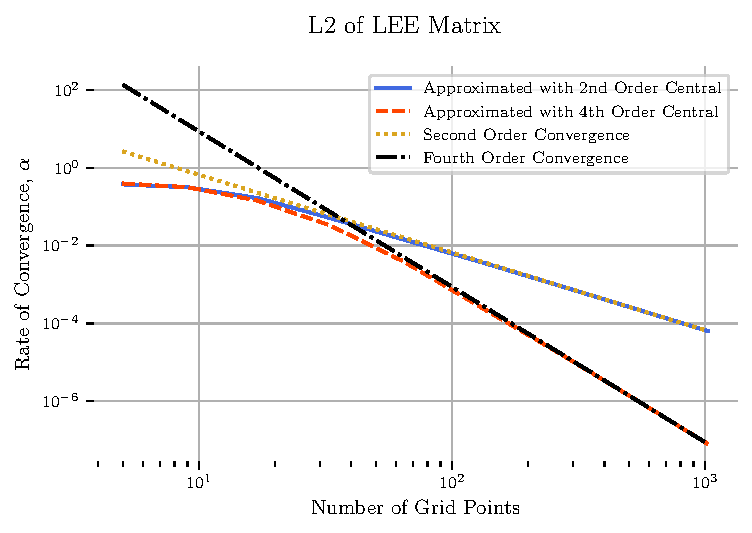
\includegraphics{/home/jeff-severino/SWIRL/CodeRun/04-plotReport/tex-outputs/MMS1_LEE_L2.pdf}
    \label{fig:9}
\end{figure}

\begin{figure}[h!]
    \centering
    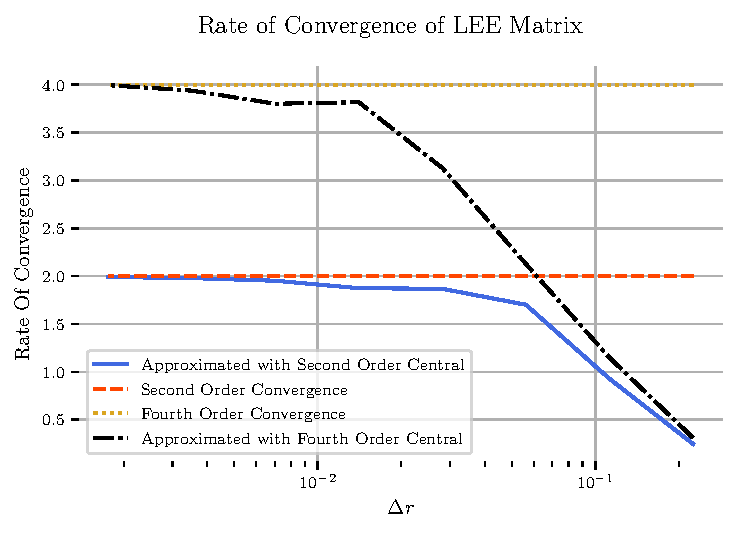
\includegraphics{/home/jeff-severino/SWIRL/CodeRun/04-plotReport/tex-outputs/MMS1_LEE_ROC.pdf}
    \label{fig:9}
\end{figure}

\newpage
\subsubsection{Test Case 1}
A comparison was conducted for a hollow cylinder undergoing uniform flow with
acoustic liners along the outer duct perimeter. The azimuthal mode number, reduced 
frequency, mach number and duct liner admittance is reported below,
\begin{align*}
    m &= 2 \\
    k &= \frac{\omega r_T}{A_T} = -1 \\
    M_x &= 0.5 \\
    \eta_T &= 0.72 + 0.42i\\
    \sigma &= 1
\end{align*} 

% \begin{figure}[h!]
%     \centering
%     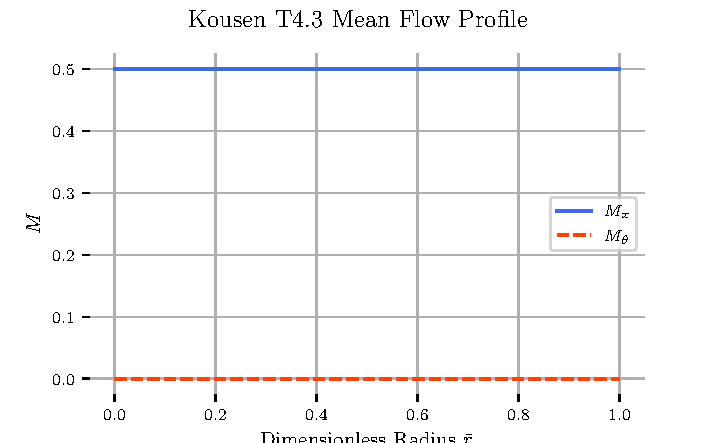
\includegraphics{/home/jeff-severino/SWIRL/CodeRun/04-plotReport/tex-outputs/KousenT1_mean_flow_profile.pdf}
%     \caption{Mean mach number profile for the uniform flow in a lined cylinder}
%     \label{fig:1}
% \end{figure}


\begin{figure}[h!]
    \centering
    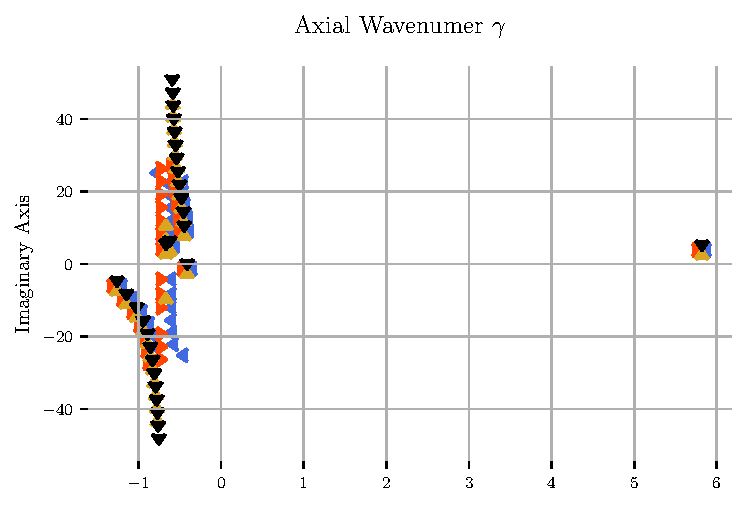
\includegraphics[width=\textwidth]{/home/jeff-severino/SWIRL/CodeRun/04-plotReport/tex-outputs/KousenT1_gam_nonconv_scatter_2ndOrderApprox.pdf}
\end{figure}



% \begin{figure}[h!]
%     \centering
%     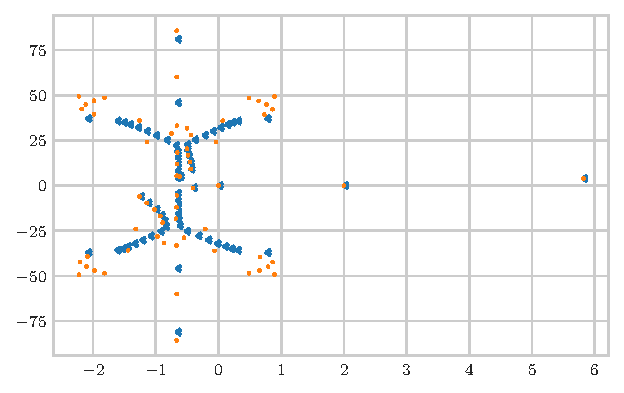
\includegraphics[width=\textwidth]{/home/jeff-severino/SWIRL/CodeRun/04-plotReport/tex-outputs/gam.nonconv.scatter_2nd_ord_32pts.pdf}
% \end{figure}

% \begin{figure}[h!]
%     \centering
%     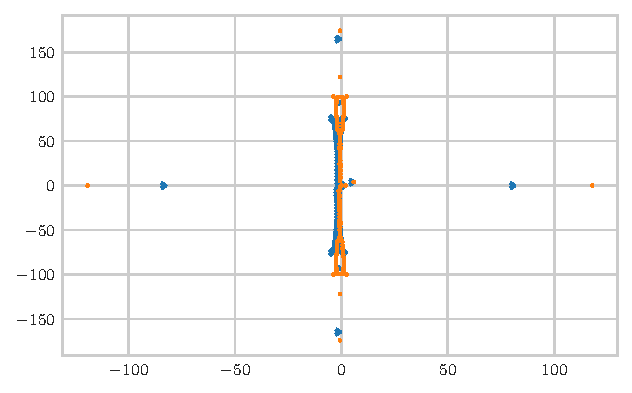
\includegraphics[width=\textwidth]{/home/jeff-severino/SWIRL/CodeRun/04-plotReport/tex-outputs/gam.nonconv.scatter_2nd_ord_64pts.pdf}
% \end{figure}


% \begin{figure}[h!]
%     \centering
%     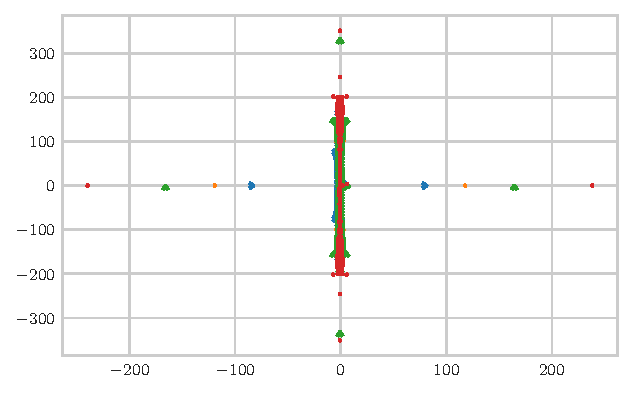
\includegraphics[width=\textwidth]{/home/jeff-severino/SWIRL/CodeRun/04-plotReport/tex-outputs/gam.nonconv.scatter_2nd_ord_128pts.pdf}
% \end{figure}

\begin{figure}[h!]
    \centering
    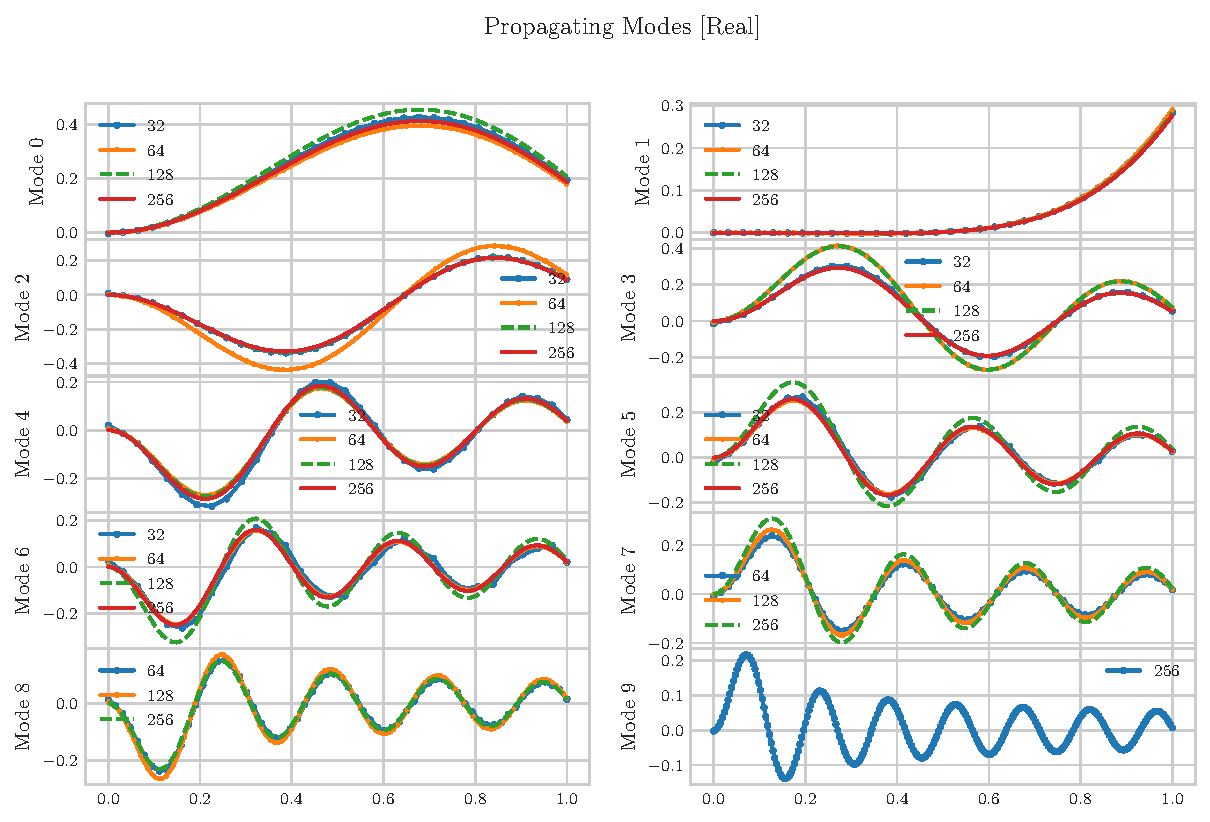
\includegraphics[width=\textwidth]{/home/jeff-severino/SWIRL/CodeRun/04-plotReport/tex-outputs/egv_prop_re.pdf}
    \label{fig:prop_re}
\end{figure}

\begin{figure}[h!]
    \centering
    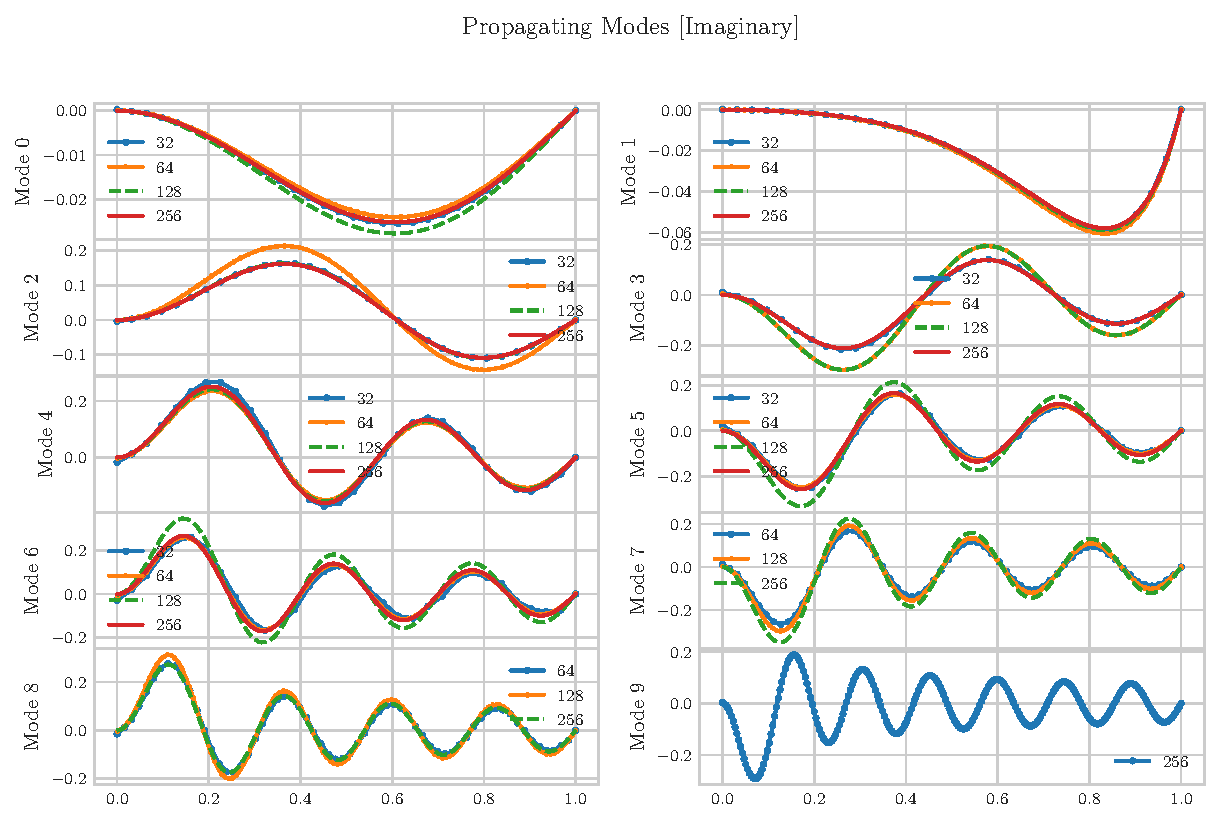
\includegraphics[width=\textwidth]{/home/jeff-severino/SWIRL/CodeRun/04-plotReport/tex-outputs/egv_prop_im.pdf}
    \label{fig:prop_im}
\end{figure}

\begin{figure}[h!]
    \centering
    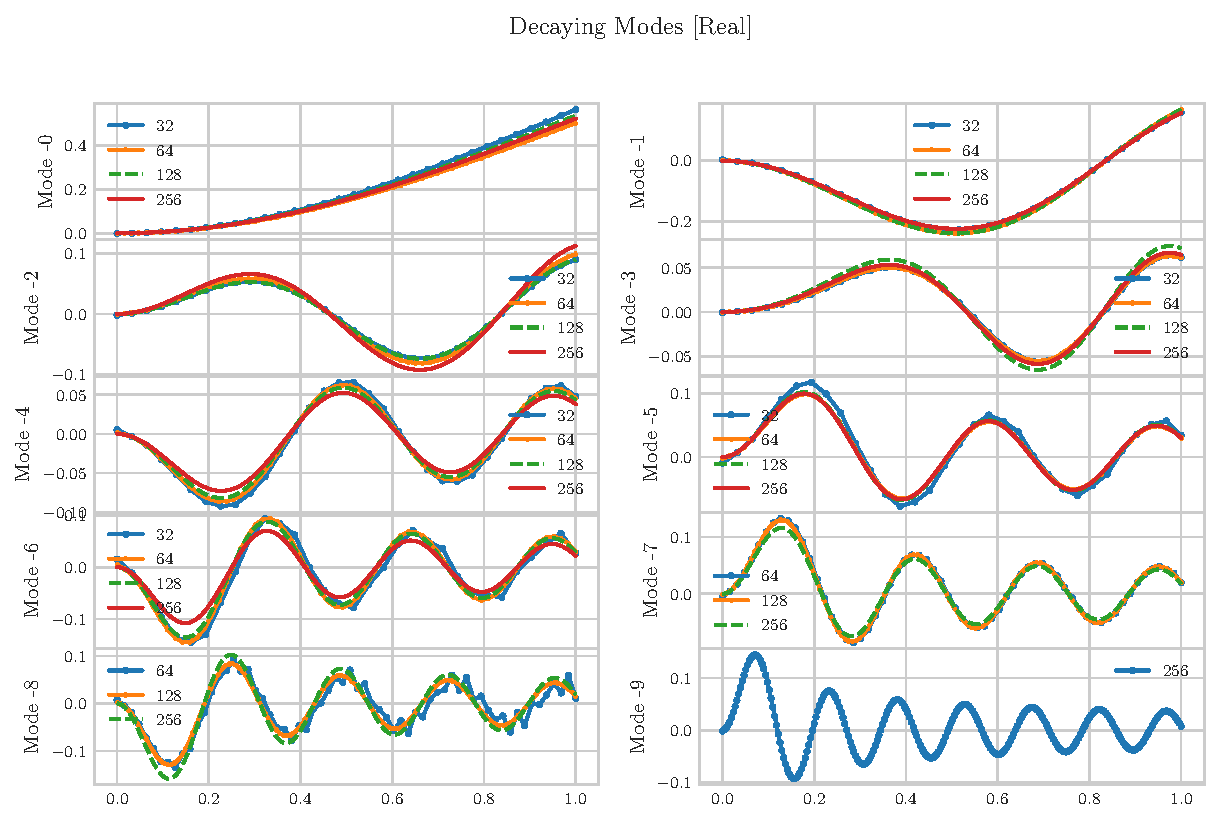
\includegraphics[width=\textwidth]{/home/jeff-severino/SWIRL/CodeRun/04-plotReport/tex-outputs/egv_decay_re.pdf}
    \label{fig:decay_re} 
\end{figure}

\begin{figure}[h!]
    \centering
    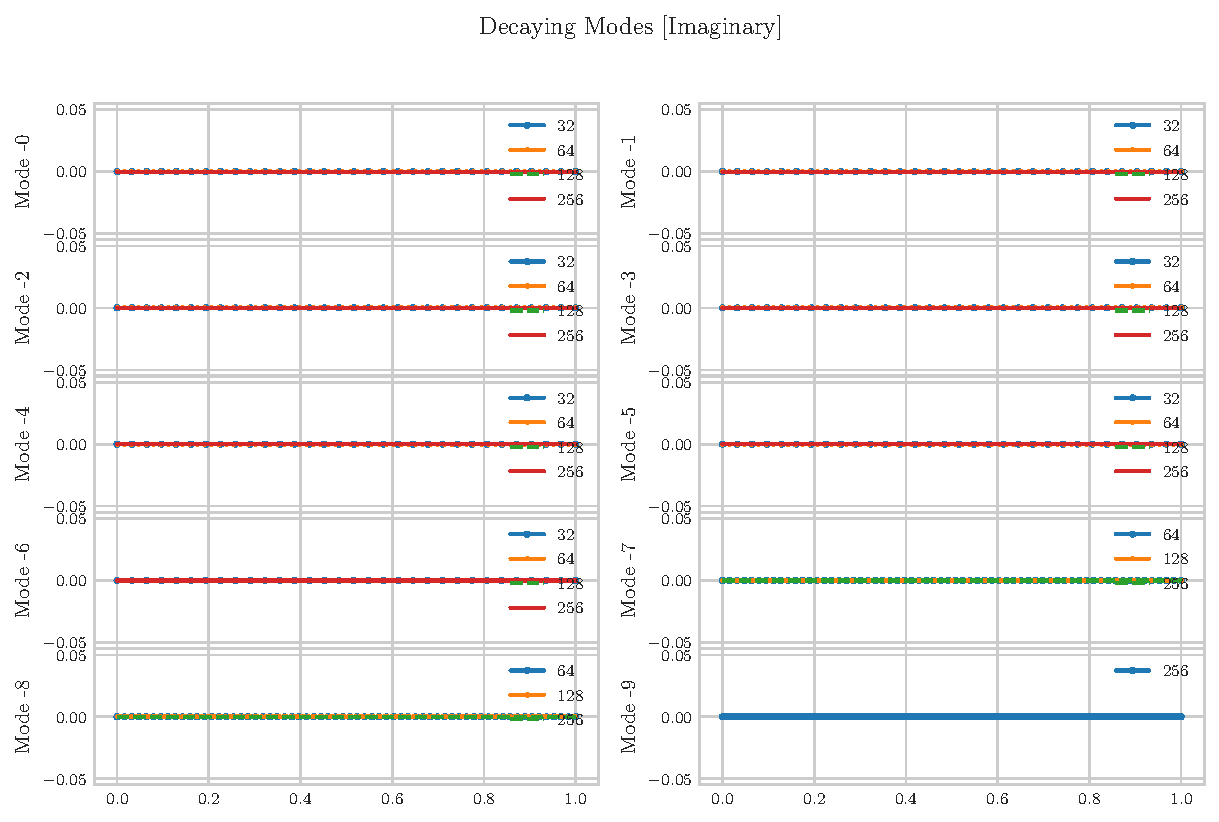
\includegraphics[width=\textwidth]{/home/jeff-severino/SWIRL/CodeRun/04-plotReport/tex-outputs/egv_decay_im.pdf}
    \label{fig:decay_im} 
\end{figure}








The results shown in \ref{Table43} are in moderately good agreement. The 
results were obtained by visually comparing the output for 32 
grid points. Note that the indicies for the SWIRL deliverable are different that 
the ones obtained for the most recent version of the code. While the 
convective axial wavenumbers show agreement to machine precision, this is not 
particularly insightful given that there are an infinite number of possible solutions 
that could satisfy the eigenvalue problem. The results that are of concern 
are propagating modes that are not convecting with the mean flow.  The scatter plot
of the axial wavenumbers show some sporadic behaviour around the imaginary axis.
The results from the MMS along with this plot indicate that more grid points are going 
to be needed if a finite difference technique is to be used.

The first 10 propagating and decaying modes are plotted in \ref{fig:prop_re}-\ref{fig:decay_im}.



% It should be 
% noted that a spectral differencing method were using for Kousen's report and for
% srcF2008. 
%Using a higher order scheme would also improve accuracy.


\begin{table}
 \centering
 \begin{adjustbox}{width=1\textwidth}
     \small
\begin{tabular}{c | r | r | r }
 \hline
 $\gamma^{\pm}_n$ & Kousen Ref. [15] & Kousen report &   current  \\
 \hline
 $\gamma_0^{+}$ & $ 0.620 - 5.014  i $ & $ 0.6195 - 5.0139 i$ & 0.620755853112 - 5.00592416941i  \\
 $\gamma_1^{+}$ & $-5.820 - 3.897  i $ & $-5.8195 - 3.8968 i$ &-0.581267772517 - 3.90050864568i \\
 $\gamma_2^{+}$ & $ 0.445 - 9.187  i $ & $ 0.4453 - 9.1868 i$ &0.451569491142 -  9.12191317214i\\
 $\gamma_3^{+}$ & $ 0.453 - 13.062 i $ & $ 0.4539 - 13.062 i$ &0.464247902898 - 12.8487472519i \\ 
 $\gamma_4^{+}$ & $ 0.480 - 16.822 i $ & $ 0.4795 - 16.822 i$ &0.492340380223 - 16.3292825150i \\
 % $\gamma_5^{+}$ & $ 0.503 - 20.531 i $ & $ 0.5029 - 20.531 i$ &0.514522630594 -19.5817182568i \\
 % $\gamma_6^{+}$ & $ 0.522 - 24.213 i $ & $ 0.5220 - 24.213 i$ &0.516658239854 -22.5715880605i \\
 % $\gamma_7^{+}$ & $ 0.538 - 27.880 i $ & $ 0.5376 - 27.880 i$ & -  \\
 % $\gamma_8^{+}$ & $ 0.550 - 31.537 i $ & $ 0.5502 - 31.537 i$ & -  \\
 % $\gamma_9^{+}$ & $ 0.589 - 49.75  i $ & $ 0.5891 - 49.754 i$ &-  \\ \hline
 $\gamma_0^{-}$ & $ 0.410 + 1.290  i $ & $ 0.4101 + 1.2904 i$ &0.409973310292  + 1.29020083859i\\
 $\gamma_1^{-}$ & $ 1.259 + 6.085  i $ & $ 1.2595 + 6.0852 i$ &1.25530612217  + 6.07214375548i \\
 $\gamma_2^{-}$ & $ 1.146 + 9.668  i $ & $ 1.1457 + 9.6679 i$ &1.13696444935  + 9.59622801724i \\
 $\gamma_3^{-}$ & $ 1.022 + 13.315 i $ & $ 1.0218 + 13.315 i$  &1.00950576515 + 13.0957277529i \\
 $\gamma_4^{-}$ & $ 0.943 + 16.977 i $ & $ 0.9425 + 16.977 i$  &0.928059983039 +  16.4791343118i\\ \hline
 % $\gamma_5^{-}$ & $ 0.891 + 20.635 i $ & $ 0.8908 + 20.635 i$    &0.856678172769 +  22.6544943903i \\
 % $\gamma_6^{-}$ & $ 0.855 + 24.288 i $ & $ 0.8549 + 24.288 i$    &0.941762848775 +  25.3460188358i \\
 % $\gamma_7^{-}$ & $ 0.829 + 27.937 i $ & $ 0.8288 + 27.937 i$    &-  \\
 % $\gamma_8^{-}$ & $ 0.809 + 31.581 i $ & $ 0.8089 + 31.581 i$    &-  \\
 % $\gamma_9^{-}$ & $ 0.755 + 49.77  i $ & $ 0.7547 + 49.772 i$    &-  \\ \hline
 \end{tabular}
\end{adjustbox}
\caption{Cylindical duct with Uniform flow, $M_x = 0.5$ and Acoustic Liner $\eta_{T} = 0.72 + 0.42i$, $k = -1$, and $m=2$}
 \label{Table43}
\end{table}


\newpage
\section{Sheared Flow Results}

The axial Mach number for these sheared flow validation cases were taken to be,

\begin{align}
    M_x = M_0 \left( 1 - \bar{r}_{Shankar} \right)^{ \frac{1}{7}}
    \label{eqn:cylindricalShear} \\
\end{align}

where $\bar{r}_{Shankar} = \frac{r_{min}}{r_{max}-r_{min}} = \frac{r_{min}}{b}$ 

Since the radius is non-dimensionalized differently in \ref{Shankar1972}, the 
velocity profile defined as a function of $\bar{r}_{Shankar}$.


\begin{figure}[h!]
    \centering
    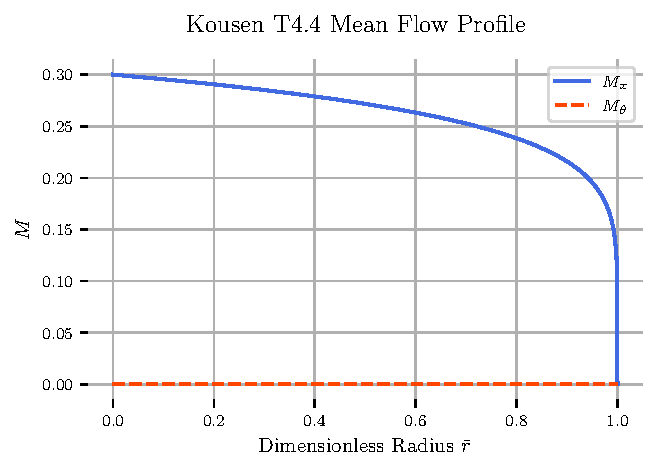
\includegraphics{/home/jeff-severino/SWIRL/CodeRun/04-plotReport/tex-outputs/KousenT2_mean_flow_profile.pdf}
    \caption{Mean mach number profile for the uniform flow in a lined cylinder}
    \label{fig:1}
\end{figure}


\newpage
\section{Sheared Flow Results}

The axial Mach number for these sheared flow validation cases were taken to be,

\begin{align}
    M_x = M_0 \left( 1 - \bar{r}_{Shankar} \right)^{ \frac{1}{7}}
    \label{eqn:cylindricalShear} \\
\end{align}

where $\bar{r}_{Shankar} = \frac{r_{min}}{r_{max}-r_{min}} = \frac{r_{min}}{b}$ 

Since the radius is non-dimensionalized differently in \ref{Shankar1972}, the 
velocity profile defined as a function of $\bar{r}_{Shankar}$.

\begin{figure}[h!]
    \centering
    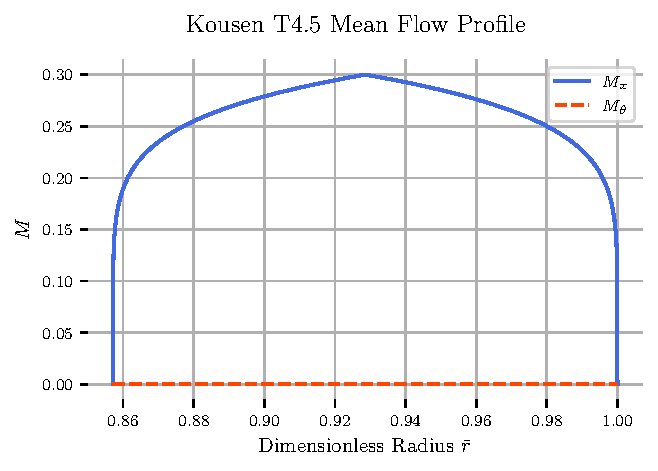
\includegraphics{/home/jeff-severino/SWIRL/CodeRun/04-plotReport/tex-outputs/KousenT3_mean_flow_profile.pdf}
    \caption{Mean mach number profile for the uniform flow in a lined cylinder}
    \label{fig:1}
\end{figure}


\newpage
\section{Sheared Flow Results}

The axial Mach number for these sheared flow validation cases were taken to be,

\begin{align}
    M_x = M_0 \left( 1 - \bar{r}_{Shankar} \right)^{ \frac{1}{7}}
    \label{eqn:cylindricalShear} \\
\end{align}

where $\bar{r}_{Shankar} = \frac{r_{min}}{r_{max}-r_{min}} = \frac{r_{min}}{b}$ 

Since the radius is non-dimensionalized differently in \ref{Shankar1972}, the 
velocity profile defined as a function of $\bar{r}_{Shankar}$.

\begin{figure}[h!]
    \centering
    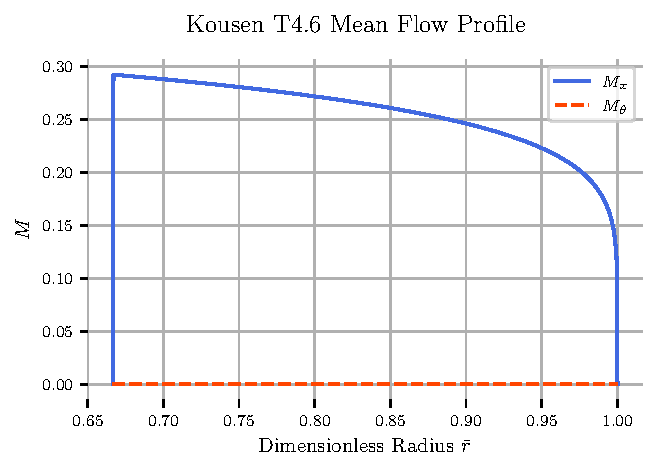
\includegraphics{/home/jeff-severino/SWIRL/CodeRun/04-plotReport/tex-outputs/KousenT4_mean_flow_profile.pdf}
    \caption{Mean mach number profile for the uniform flow in a lined cylinder}
    \label{fig:1}
\end{figure}

\begin{figure}[h!]
    \centering
    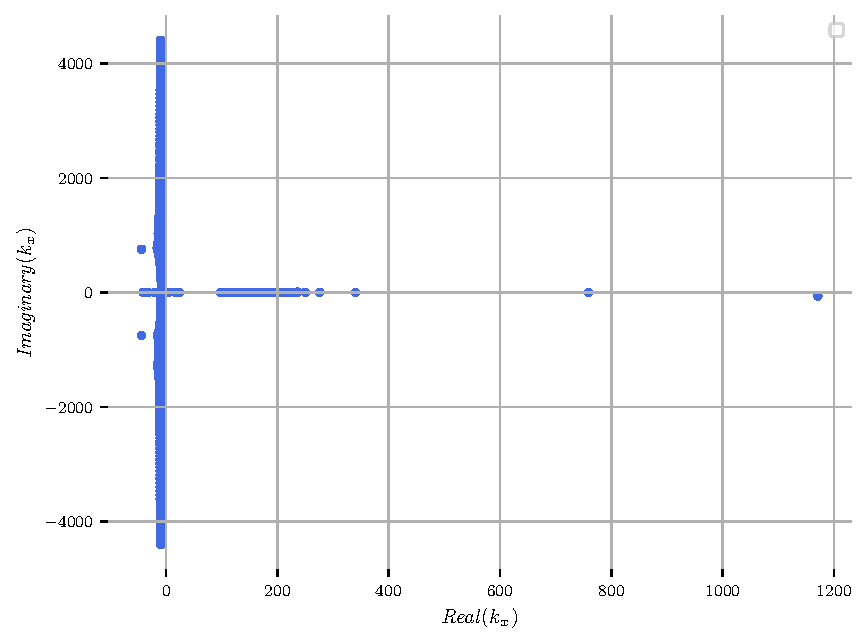
\includegraphics[width=\textwidth]{/home/jeff-severino/SWIRL/CodeRun/04-plotReport/tex-outputs/KousenT4_gam_nonconv_scatter_4thOrderApprox.pdf}
\end{figure}




% \begin{figure}[!]
%     \centering
%         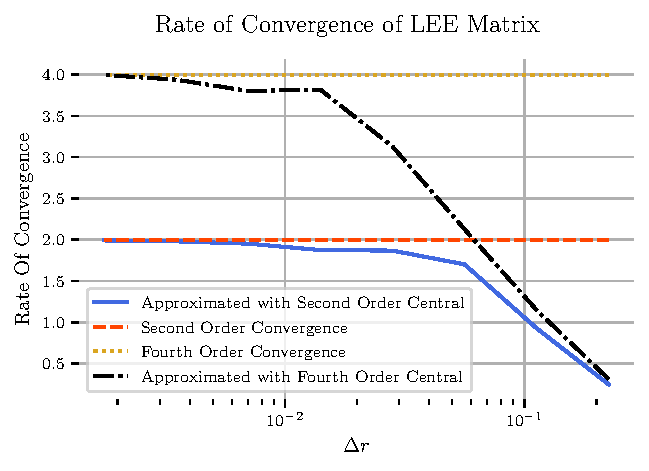
\includegraphics{/home/jeff-severino/SWIRL/CodeRun/04-plotReport/tex-outputs/LEE_ROC.pdf}
%        \caption{ROC for the LEE using second and fourth order central differencing
%        for the radial derivative}
%         \label{fig:10}
% \end{figure}





%%\begin{itemize}
%%    \item Kousen's Test Cases
%%        \subitem Cylinder, Uniform Flow with Liner (Table 4.3)
%%        \begin{align*}
%%            m &= 2 \\
%%            k &= \frac{\omega r_T}{A_T} = -1 \\
%%            M_x &= 0.5 \\
%%            \eta_T &= 0.72 + 0.42i\\
%%            \text{Confirm if 32 grid points is enough}
%%        \end{align*} 
%%        \subitem Cylinder, Shear Flow without Liner (Table 4.4)
%%        \begin{align*}
%%            m &= 0 \\
%%            kb &= \left(\frac{\omega r_T}{A_T}\right)b = 20 \\
%%            b &= r_{max} - r_{min} \\
%%            \tilde{r} = \frac{r}{b} \\
%%            M_x &= 0.3(1-\tilde{r})^{\frac{1}{7}} \\
%%            \eta_T &= 0\\
%%            \text{Confirm if 32 grid points is enough}
%%        \end{align*}
%%        \subitem Annulus, Shear Flow without Liner (Table 4.5)
%%        \begin{align*}
%%            m &= 0 \\
%%            kb &= \left(\frac{\omega r_T}{A_T}\right)b = 10 \\
%%            b &= r_{max} - r_{min}  = \frac{1}{7}\\
%%            k &= 70 \\
%%            \tilde{r} = \frac{r}{b} = 6.0 \\
%%            M_x &= 0.3\left(1 - 2 \left| \frac{r_{max}-r}{b} + 0.5 \right|  \right)^{\frac{1}{7}} \\
%%            \eta_T &= 0\\
%%            \text{Confirm if 32 grid points is enough}
%%        \end{align*}
%%        \subitem Annulus, Shear Flow with Liner (Table 4.6)
%%        \begin{align*}
%%            m &= 0 \\
%%            kb &= \left(\frac{\omega r_T}{A_T}\right)b = 10 \\
%%            b &= r_{max} - r_{min}  = \frac{1}{3}\\
%%            k &= 30 \\
%%            \tilde{r} = \frac{r}{b} = 2.0 \\
%%            M_x &= 0.3\left(1 - 2 \left| \frac{r_{max}-r}{b} + 0.5 \right|  \right)^{\frac{1}{7}} \\
%%            \eta_T &= 0.3 + 0.1i\\
%%            \text{Confirm if 32 grid points is enough}
%%        \end{align*}
%%\end{itemize}

